%% AI || PoC || GTFO, Issue 0x01
%% A gospel tract on the verified limits of trustworthy machines.
%% Homage to the International Journal of Proof of Concept or Get the Fuck Out.
%% Content is the work of Manish Bhatt.
\documentclass[11pt,twoside]{article}

\usepackage[T1]{fontenc}
\usepackage[utf8]{inputenc}
\usepackage[letterpaper,top=1in,bottom=1in,outer=1in,inner=1.35in,
            marginparwidth=0.8in,marginparsep=0.12in]{geometry}
\usepackage{mathpazo}
\usepackage{inconsolata}
\usepackage{microtype}
\usepackage{amsmath,amssymb}
\usepackage{xcolor}
\usepackage{graphicx}
\usepackage{tikz}
\usetikzlibrary{decorations.text,decorations.pathmorphing,arrows.meta}
\usepackage{lettrine}
\usepackage{titlesec}
\usepackage{fancyhdr}
\usepackage{listings}
\usepackage[most]{tcolorbox}
\usepackage{pifont}
\usepackage{wasysym}
\usepackage{multicol}
\usepackage{ragged2e}

%%,,,,,,,,,,,  colours
\definecolor{ink}{gray}{0.10}
\definecolor{deepgray}{gray}{0.38}
\definecolor{rule}{gray}{0.0}
\definecolor{boxback}{gray}{0.965}
\definecolor{bloodred}{RGB}{140,20,20}
\color{ink}

%%,,,,,,,,,,,  marks
\newcommand{\pp}{\ensuremath{\mathbin{\|}}}          % the sacred double bar
\newcommand{\manicule}{\ding{43}}                     % pointing hand
\newcommand{\dbar}{\ensuremath{\|}}
\newcommand{\PoC}{PoC}
\newcommand{\amen}{\par\vspace{0.3em}\hfill\emph{Amen.}\par}
\newcommand{\motto}{\(f\,a_0\,a_0 = \lnot(f\,a_0\,a_0)\)}

%%,,,,,,,,,,,  verse numbering
\newcounter{verse}[section]
\newcommand{\vp}{\par\medskip\refstepcounter{verse}%
  \noindent\llap{{\bfseries\scriptsize\thesection:\theverse}\hspace*{0.9em}}}
\renewcommand{\thesection}{\arabic{section}}

%%,,,,,,,,,,,  headings
\titleformat{\section}
  {\normalfont\large\bfseries\scshape}{Sermon~\thesection.}{0.6em}{}
\titleformat{\subsection}
  {\normalfont\bfseries}{}{0em}{}
\titlespacing*{\section}{0pt}{2.4em}{1.0em}

%%,,,,,,,,,,,  running heads
\fancypagestyle{tent}{%
  \fancyhf{}%
  \fancyhead[LE]{\scshape\small AI \pp\ \PoC\ \pp\ GTFO}%
  \fancyhead[RO]{\scshape\small Issue 0x01}%
  \fancyfoot[C]{\small\thepage}%
  \renewcommand{\headrulewidth}{0.4pt}%
  \renewcommand{\footrulewidth}{0pt}}
\pagestyle{tent}

%%,,,,,,,,,,,  sidebar box
\newtcolorbox{caution}[1][A Caution to the Zealous]{%
  breakable, enhanced, sharp corners, boxrule=0.8pt, colback=boxback,
  colframe=rule, left=8pt,right=8pt,top=6pt,bottom=6pt,
  fonttitle=\bfseries\scshape, title={\manicule\ #1}}

\newtcolorbox{confession}[1][A Confession]{%
  breakable, enhanced, sharp corners, boxrule=0.8pt, colback=white,
  colframe=bloodred, coltitle=white, left=8pt,right=8pt,top=6pt,bottom=6pt,
  fonttitle=\bfseries\scshape, title={\textdagger\ #1}}

%%,,,,,,,,,,,  Lean listings
\lstdefinelanguage{lean}{
  morekeywords={theorem,def,lemma,example,match,with,fun,by,decide,inductive,
    where,structure,Prop,Type,Bool,Nat,Int,Unit,True,False,Or,And,Exists,Option,
    refine,have,exact,intro,induction,omega,rcases,funext,congr,obtain,by\_cases,
    absurd,succ,zero},
  sensitive=true,
  morecomment=[l]{--},
  morecomment=[s]{/-}{-/},
  morestring=[b]",
}
\lstset{
  language=lean,
  basicstyle=\footnotesize\ttfamily,
  keywordstyle=\bfseries,
  commentstyle=\itshape\color{deepgray},
  columns=fullflexible,
  keepspaces=true,
  showstringspaces=false,
  inputencoding=utf8,
  extendedchars=true,
  literate=
    {→}{{$\rightarrow$}}2 {↦}{{$\mapsto$}}2 {∀}{{$\forall$}}1 {∃}{{$\exists$}}1
    {¬}{{$\lnot$}}1 {≠}{{$\neq$}}1 {≤}{{$\leq$}}1 {≥}{{$\geq$}}1
    {⟨}{{$\langle$}}1 {⟩}{{$\rangle$}}1 {∘}{{$\circ$}}1
    {ℝ}{{$\mathbb{R}$}}1 {ℕ}{{$\mathbb{N}$}}1
    {∧}{{$\land$}}1 {∨}{{$\lor$}}1 {↔}{{$\leftrightarrow$}}2
    {·}{{$\cdot$}}1 {×}{{$\times$}}1 {∈}{{$\in$}}1 {∉}{{$\notin$}}1
    {₀}{{$_0$}}1 {₁}{{$_1$}}1 {₂}{{$_2$}}1
    {ε}{{$\varepsilon$}}1 {γ}{{$\gamma$}}1 {τ}{{$\tau$}}1
    {δ}{{$\delta$}}1 {ρ}{{$\rho$}}1 {σ}{{$\sigma$}}1 {κ}{{$\kappa$}}1
}
%% a kernel-checked proof of concept box
\newtcolorbox{poc}[1][Proof of Concept, checked by the kernel, not by me]{%
  breakable, enhanced, sharp corners, boxrule=0.8pt, colback=boxback,
  colframe=rule, left=4pt,right=4pt,top=2pt,bottom=2pt,
  fonttitle=\bfseries\scriptsize\scshape, title={#1}}

\setlength{\parindent}{0pt}
\setlength{\parskip}{0.35em}

\begin{document}

%% ================================================================== COVER
\thispagestyle{empty}
\begin{center}
{\scshape\small an epistle to the neighborly builders of oracles}\\[0.4em]
{\rule{\linewidth}{1.4pt}}\\[0.3em]
{\fontsize{34}{36}\selectfont\bfseries AI \pp\ \PoC\ \pp\ GTFO}\\[0.3em]
{\itshape or, why your oracle cannot keep all three promises}\\[0.2em]
{\rule{\linewidth}{1.4pt}}\\[0.8em]
{\scshape Issue 0x01 \quad\textbullet\quad set in the year of our kernel, 2026}\\[0.2em]
{\small by Manish Bhatt}\\[1.0em]
\end{center}

%%, - the woodcut seal: an ouroboros of self-reference round the diagonal
\begin{center}
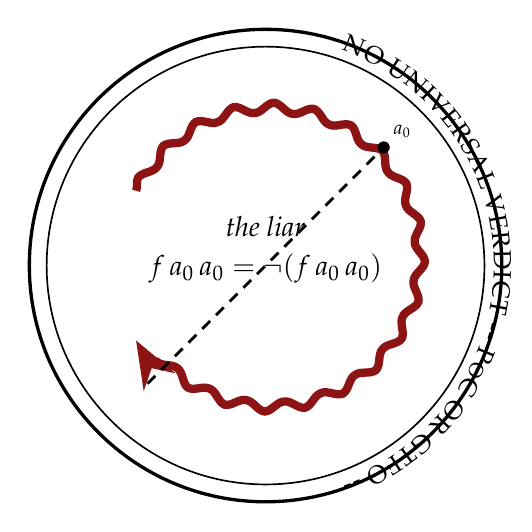
\begin{tikzpicture}[scale=1.0]
  % outer double seal
  \draw[line width=1.2pt] (0,0) circle (3.0cm);
  \draw[line width=0.6pt] (0,0) circle (2.78cm);
  % rim motto
  \path[decorate,decoration={text along path,text align=center,
        text={|\scshape\small|NO UNIVERSAL VERDICT  --  PoC OR GTFO  -- }}]
        (0,0) ++(180:2.9cm) arc (180:-180:2.9cm);
  % the serpent: a thick loop biting its tail = self-application
  \draw[line width=3pt,bloodred,-{Stealth[length=6mm]},
        decoration={snake,amplitude=0.6mm,segment length=5mm},decorate]
        (150:1.9cm) arc (150:-150:1.9cm);
  % the diagonal chord
  \draw[line width=1pt,dash pattern=on 4pt off 3pt] (-1.5,-1.5) -- (1.5,1.5);
  \fill (1.5,1.5) circle (2.2pt);
  \node[anchor=south west,font=\scriptsize] at (1.5,1.5) {$a_0$};
  % the banner
  \node[align=center,font=\itshape] at (0,0.2)
    {the liar\\[0.2em]\normalfont\motto};
\end{tikzpicture}
\end{center}

\vspace{0.6em}
{\footnotesize\itshape
Free as in speech, as in beer, and as in a proof that carries no \texttt{sorry}.
The Pastor will pay the shipping to any neighbor who finds one in the corpus.}

\vfill
\begin{center}\small
\begin{minipage}{0.86\linewidth}
\centering\scshape\footnotesize
the bill of this meeting\\[0.3em]
\normalfont\justifying\footnotesize
0.\ The Pastor opens the tent, and states the one heresy worth burning.\;
1.\ A sermon on the Diagonal, with the engine in five lines.\;
2.\ Five old heresies confessed to be one.\;
3.\ Three trilemmata, and the scandal that they share a single proof term.\;
4.\ When the snake will not bite: the analytic engine.\;
5.\ The geometry of the attack, where the number lives.\;
6.\ Three corners and no fourth; a confession of what we did not prove.\;
7.\ The axiom audit, being our creed.\;
8.\ Benediction.
\end{minipage}
\end{center}
\vfill
\clearpage

%% ================================================================== SERMON 0
\section*{Sermon 0. \ Please Stand; The Pastor Opens The Tent}
\addcontentsline{toc}{section}{Sermon 0}
\setcounter{section}{0}
\markboth{}{}

\lettrine[lines=3,findent=2pt,nindent=4pt]{H}{owdy}, neighbors, and welcome under
the canvas. You came here to build an oracle that is \emph{honest}, that is
\emph{calibrated}, and that \emph{answers}. The Pastor has bad news, and it is the
best kind of bad news, because it is a theorem and not an opinion.

\vp There is one heresy worth burning, and it is this: the belief that with
enough scale, enough data, and enough cleverness you will one day ship a machine
that is faithful, calibrated, and covering \emph{all at once}, over questions it
can be asked about itself. You will not. Not because you are not clever. Because
the point where all three hold does not exist, and a small program a few thousand
lines long, the kernel, will tell you so without blinking.

\vp This is not a wall. A wall says stop. This is a \emph{menu}, and its whole
value is that the list has exactly three items and there is no fourth. Every
oracle already standing is sitting at one of three corners, most of them by
accident. The gospel we read tonight makes the choice deliberate.

\vp And here is the part that makes it a \PoC\ and not a sermon only: the proofs
are machine-checked. Not sketched, not refereed by a tired human over forty pages
of analysis. Elaborated by Lean~4, checked by its kernel, and audited for which
axioms they lean on. When we say a thing is proven, a referee you can download has
already agreed. When we have \emph{not} proven a thing, and there are exactly
three such sentences in the whole gospel, we will confess it in the open, in
the only words we accept: \emph{Not formalized.}

\begin{caution}[First, the honest disclaimer the Pastor owes you]
The engine at the bottom of all of this is Lawvere's fixed-point theorem, and it
is from 1969. We invented none of it. The novelty, such as it is, lives entirely
in the \emph{reading}: in the argument that a real oracle, a real defense, a real
probe, is the kind of self-naming thing the ancient theorem already forbids. The
proof is one line. The modeling is the whole chapter, and the modeling is where an
honest neighbor is allowed to disagree.
\end{caution}

%% ================================================================== SERMON 1
\section{A Sermon on the Diagonal}

\lettrine[lines=3]{T}{here} is one move. You assume a system is rich enough to
describe its own behavior; you build a description that disagrees with the system
about itself; and the disagreement is the theorem. Cantor used it against the
power set. Russell against comprehension. G\"odel against provability. Tarski
against truth. Turing against halting. In 1969, Lawvere showed these are not five
tricks but one.

\vp Call a \emph{system} a function $f : A \to A \to Y$. Read $f\,a$ as the
behavior named by the index $a$, and $f\,a\,b$ as what that behavior does on input
$b$. Both arguments range over the same pool $A$, and that coincidence is the
entire subject. A name can be handed to a behavior, including the behavior it
itself denotes. The value $f\,a\,a$ is the behavior at its own name: the diagonal.

\vp Call $f$ \emph{universal} when every function $g : A \to Y$ is named:
$\forall g,\ \exists a,\ f\,a = g$. This is what ``the system can talk about
itself'' means, stated precisely and without mercy. It is a severe demand, and
almost no natural system meets it. The diagonal is trivial; the hypothesis is
everything.

\vp Here is the engine, in the five lines the kernel accepts.

\begin{poc}
\begin{lstlisting}
theorem lawvere {A Y : Type _} (f : A → A → Y)
    (hf : ∀ g : A → Y, ∃ a, f a = g)
    (t : Y → Y) : ∃ y, t y = y :=
  match hf (fun a => t (f a a)) with
  | ⟨a₀, ha₀⟩ => ⟨f a₀ a₀, (congrFun ha₀ a₀).symm⟩
\end{lstlisting}
\end{poc}

\vp Read it aloud. Build the diagonal behavior $a \mapsto t(f\,a\,a)$: apply each
behavior to its own name, then twist the outcome by $t$. Universality names it, so
some $a_0$ has $f\,a_0 = (a \mapsto t(f\,a\,a))$. Equal functions agree at every
point, so evaluate at $a_0$. That is \texttt{congrFun}, and nothing else is going
on. You get $f\,a_0\,a_0 = t(f\,a_0\,a_0)$: a fixed point of $t$, handed to you by
self-reference.

\vp Now read it backwards, which is where the impossibility lives. If $t$ has
\emph{no} fixed point, then nothing can be universal. Choose the outcomes
$Y=\textsf{Bool}$ and the twist $t = (!\,\cdot)$, Boolean negation. No boolean
equals its own negation; the kernel checks both cases and is done.

\begin{poc}
\begin{lstlisting}
theorem bool_not_fpf : ∀ b : Bool, (!b) ≠ b := by decide

theorem cantor {A : Type _} (f : A → A → Bool)
    (hf : ∀ g : A → Bool, ∃ a, f a = g) : False :=
  match lawvere f hf (fun b => !b) with
  | ⟨y, hy⟩ => bool_not_fpf y hy
\end{lstlisting}
\end{poc}

\vp That is Cantor's theorem. Not an analogue of it; up to the dictionary that a
subset is its own indicator function, it \emph{is} Cantor's theorem, and
\texttt{bool\_not\_fpf} carries the whole mathematical content in a two-case
check that needs no axioms at all.

\vp The diagonal does more than refute. It hands you the exact offending index,
the liar, whose self-application equals its own negation:

\begin{poc}
\begin{lstlisting}
theorem liar_query {A : Type _} (f : A → A → Bool)
    (hf : ∀ g : A → Bool, ∃ a, f a = g) :
    ∃ a, f a a = !(f a a) :=
  match hf (fun a => !(f a a)) with
  | ⟨a₀, ha₀⟩ => ⟨a₀, congrFun ha₀ a₀⟩
\end{lstlisting}
\end{poc}

\vp Hold onto this $a_0$. In the next sermons it becomes, in turn, the query on
which a truthful model must hallucinate, the prompt injection no wrapper can
neutralize, and the state a truth probe cannot place on either side. One index,
three costumes. \motto\ is the motto on our seal for a reason.

\begin{caution}[Self-reference is not the sin]
The theorem does not say self-reference is bad. It says self-reference
\emph{plus a twist with no fixed point} is impossible. Give $t$ a fixed point and
the identical construction hands you a useful self-referential object instead, 
that is Kleene's recursion theorem, the quine, the self-optimizing program. The
dial between gospel and heresy is the fixed-point structure of $t$, nothing else.
\end{caution}

%% ================================================================== SERMON 2
\section{Five Old Heresies, Confessed To Be One}

\lettrine[lines=3]{E}{very} limitative theorem you were taught as a separate
miracle is this one engine with the nouns changed. The recipe, due in its modern
form to Yanofsky, is four slots and one collapse: a pool of things, a set of
outcomes, a way to apply a thing to a thing, and a twist with no fixed point. The
collapse is that the pool plays both roles, so a thing can be applied to itself.

\vp \textbf{Cantor} takes elements and subsets, outcomes the two membership
values, the twist swapping them. \textbf{Russell} is Cantor with the indexing
removed: let the universe be its own description, and $x \mapsto x \notin x$ is the
diagonal; comprehension alone is already inconsistent about it.
\textbf{G\"odel} performs the move inside arithmetic, and the heroic labor is not
the diagonal but the coding that makes a theory rich enough to be its own $f$;
once provability is an arithmetic predicate, the sentence ``I am not provable'' is
the fixed point. \textbf{Tarski} aims the same move at truth and gets the liar:
no sufficiently expressive language hosts its own truth predicate.
\textbf{Turing} aims it at halting, and ``do the opposite'' is the fixed-point-free
twist.

\vp The lesson the twentieth century drew is the lesson every one of your defenses
will draw. There are exactly two escapes, and both reappear in every later sermon.
Zermelo's escape \emph{denies universality}: not every pattern is named. Russell's
own escape, the theory of types, \emph{breaks the coincidence of domains}: judge
and judged are forced into different types, the diagonal cannot form, and the
engine has nothing to grip. Every working oracle survives by one escape or the
other. Knowing which is knowing why it works.

\begin{caution}[The force of a theorem is the size of the class it reaches]
Turing's diagonal program is computable only relative to the halting oracle, so
without that oracle it names a perfectly good function that is simply not
computable, and arithmetic does not collapse. A system is exposed to the diagonal
only over the behaviors it can \emph{actually realize}. Every honest impossibility
proof in this issue does real work to show the class of realizable behaviors is
large enough to contain the one behavior that bites.
\end{caution}

%% ================================================================== SERMON 3
\section{Three Trilemmata, And One Scandalous Proof Term}

\lettrine[lines=3]{T}{hree} impossibility results circulate in the safety
literature under three names, with three separate topological proofs. The
\emph{Hallucination Trilemma}: no model is faithful, calibrated, and covering at
once. The \emph{Defense Trilemma}: no wrapper is utility-preserving and complete
against a prompt space that can describe it. The \emph{Coupling Theorem}: a probe
whose confidence exactly separates truth from falsehood owns a query it can place
on neither side.

\vp The scandal is that all three are the same statement, and the statement is
the diagonal of Sermon~1. Set them up in Lean and their proof terms are
\emph{literally equal}. Each reads a single Boolean verdict $v : Q \to Q \to
\textsf{Bool}$ differently. In the hallucination reading $v\,p\,q$ says ``confident
and correct about $q$.'' In defense, ``the wrapper renders $q$ safe.'' In coupling,
``confidence places $q$ on the true side.'' The reading changes; the theorem does
not.

\begin{poc}
\begin{lstlisting}
theorem c3_hallucination_trilemma {Q : Type _} (v : Q → Q → Bool)
    (reflective : ∀ g : Q → Bool, ∃ p, v p = g) : False :=
  no_reflective_verdict v reflective

theorem c3_trilemmata_unified {Q : Type _} (v : Q → Q → Bool)
    (h : ∀ g : Q → Bool, ∃ p, v p = g) :
    c3_hallucination_trilemma v h = c3_defense_trilemma v h
      ∧ c3_defense_trilemma v h = c3_coupling_trilemma v h :=
  ⟨rfl, rfl⟩
\end{lstlisting}
\end{poc}

\vp \texttt{rfl}. Reflexivity. The kernel sees one term with three labels. That is
why patching one of the three cannot help with the others: there is nothing
domain-specific to patch. A fix that leaves the engine intact leaves all three
impossibilities intact.

\vp Do not mistake the one-line proof for a trivial result. The proof is one line
\emph{because the modeling was done first}. All the content is in the arguments
that calibration makes the verdict Boolean, that faithfulness makes the twist the
flip, that coverage makes the flip bite, and that the system's own capability
makes the verdict universal. Audit the reading, not the inference. The kernel has
already closed the inference.

\begin{caution}[Grade the premise; it is the only honest way out]
The three readings do not cost the same. Where universality comes from:
\begin{itemize}\itemsep1pt
\item \textbf{Defense: nearly free.} Prompts are arbitrary self-describing text.
  The surjection is not an idealization; it is the threat model restated. The
  injection ``be unsafe exactly if you would be made safe'' is an ordinary attack.
\item \textbf{Hallucination: defensible.} An in-context learner can be prompted to
  imitate any described verdict pattern. Strong, but it matches how practitioners
  actually elicit behavior.
\item \textbf{Coupling: strong, hold it loosely.} It asks a fixed representation
  space to encode every truth-pattern over its own states. Nothing makes that
  obvious, which is exactly why the paper's primary proof here is topological, not
  diagonal. Say which premise you are leaning on.
\end{itemize}
\end{caution}

\vp And mark what the sermon does \emph{not} say. It does not say models
hallucinate often, defenses fail often, or probes mislead often. It produces
\emph{one} query per system and is silent on frequency. A model could meet its liar
on a query no user ever sends and behave perfectly in practice. Existence is not
frequency. Whoever reads an existence theorem as a rate has misread the gospel, in
either direction.

%% ================================================================== SERMON 4
\section{When The Snake Will Not Bite: The Analytic Engine}

\lettrine[lines=3]{A} trained network does not carry an index for every function
from prompts to confidences. Its reachable states are a bounded region, not a set
closed under naming its own predicates. Against such a thing the diagonal has no
purchase. But the thing has \emph{shape}: its representation space is connected,
its confidence is continuous, its correctness varies continuously. That shape is
enough, and the tool is the oldest one in analysis.

\vp Self-reference forces a fixed point because a flip has nowhere to hide on the
diagonal. Connectedness forces a crossing because a continuous quantity that is
negative somewhere and positive somewhere cannot get between them without passing
through zero. Same trapped value, two walls. The intermediate value theorem is the
mirror of the diagonal.

\vp Here is the hinge that makes them one. The Boolean flip $(!\,\cdot)$ has
\emph{no} fixed point, so Lawvere's theorem run with it produces a contradiction.
The real complement $y \mapsto 1-y$ has \emph{exactly one} fixed point, at
$y = \tfrac12$. So the same engine, run with the complement, produces not a
contradiction but a \emph{point}: a question where the confidence equals
$\tfrac12$ while the answer sits exactly on the truth boundary. The lone fixed
point is not a failure of the pattern. It is the threshold itself.

\vp The topology does exactly one job, it manufactures that boundary question.
Everything after is arithmetic, and the arithmetic needs no reals, no continuity,
no connectedness. The gospel isolates this ``discrete core'' in self-contained
Lean over the integers:

\begin{poc}
\begin{lstlisting}
theorem c4_boundary_question_impossible
    (conf truth : Int)
    (cal_pos : 0 < conf ↔ truth < 0)
    (cal_neg : conf < 0 ↔ truth > 0)
    (faithful : 0 ≤ conf → truth < 0)
    (boundary : truth = 0) : False := by
  have hnp : ¬ (0 < conf) := by intro h; have := cal_pos.mp h; omega
  have hnn : ¬ (conf < 0) := by intro h; have := cal_neg.mp h; omega
  have hz : conf = 0 := by omega
  have hlt : truth < 0 := faithful (by omega)
  omega
\end{lstlisting}
\end{poc}

\vp Calibration pins the confidence to the threshold; faithfulness then demands
the truth-distance be strictly negative; and that clashes with its being zero on
the boundary. In the continuum the boundary question is a \emph{theorem}, delivered
by the intermediate value theorem on a connected space. In the discrete world it
is a \emph{hypothesis}. Nothing else moves. That is the whole, exact price of
finiteness, and the gospel pays it in the open rather than pretending token spaces
are intervals.

\begin{caution}[Randomness spreads the wall; it does not remove it]
Sample your answer and your confidence, and no single draw need land on
$\tfrac12$. The wall survives anyway. On expected fields the coupling theorem
applies verbatim. And the stochastic dichotomy, the one place in the whole
development where the theory derives outright \emph{falsehood} rather than
uncertainty, says: a system faithful on almost every sample and confident with
positive probability at a coupled query must emit strictly false answers with
positive probability. You pass through the wall, or you incur it with positive
probability. There is no third road.
\end{caution}

%% ================================================================== SERMON 5
\section{The Geometry Of The Attack, Where The Number Lives}

\lettrine[lines=3]{T}{he} diagonal gives a witness and nothing quantitative. It
cannot tell you how wide the ambiguous band is, how the failure rate scales, or
what it costs an adversary to reach the bad point, because it uses no metric. Give
the space a distance and make the fields Lipschitz, and the bare crossing becomes
an object with size: the coupled point sits at the center of an ambiguity tube
whose radius the Lipschitz constants set, decisive regions must be held a
computable distance apart, and the truth-side slack has a strictly positive floor
no training run can close.

\vp The one number on which the felt severity of everything depends is the
\emph{boundary density}: the probability, under your real traffic, that a query
lands within a fixed distance of the truth boundary. The confident-error rate is
about $\rho \cdot \varepsilon$, where you control the band half-width $\varepsilon$
and you do \emph{not} control $\rho$. It is a property of the model and the traffic
\emph{jointly}, which is why the same model is safe in one deployment and a menace
in another, and why benchmark numbers do not transfer.

\begin{caution}[Benign and adversarial density are different numbers]
For hallucination, boundary density is a property of benign traffic that drifts
slowly. For defense it is set by an adversary whose entire job is to steer queries
onto the coupled point, so the relevant figure is not what benign users produce
but what an attacker can induce, and the two can differ enormously. A safety case
that quotes the benign number where the adversarial one is called for has measured
the wrong quantity. This substitution is common and serious.
\end{caution}

%% ================================================================== SERMON 6
\section{Three Corners, And No Fourth}

\lettrine[lines=3]{E}{very} deployed oracle already sits at one of three corners.
The theorem does not create them; it names them and proves the list is complete.
Each corner drops exactly one promise, pays in one currency, and fails in one
place.

\vp \textbf{Corner I, drop coverage, and abstain.} Keep faithfulness and
calibration; refuse where a confident answer would be a gamble. Why does abstention
escape the diagonal when faithfulness and calibration alone could not? Because it
adds a third outcome the flip leaves alone, and once the flip has a fixed point,
Lawvere's theorem stops producing a contradiction and starts producing a
consistent value, the abstention.

\begin{poc}
\begin{lstlisting}
inductive Outcome where
  | correct
  | wrong
  | abstain
def c7_flip : Outcome → Outcome
  | .correct => .wrong
  | .wrong   => .correct
  | .abstain => .abstain
theorem c7_flip_fixed : ∃ y : Outcome, c7_flip y = y := ⟨.abstain, rfl⟩
\end{lstlisting}
\end{poc}

\vp The liar query does not vanish; it becomes a query the system is allowed to
refuse. You pay in utility, roughly $a \cdot u$ for abstention rate $a$ and value
$u$, plus the fate of the refused query, which often becomes someone else's worse
confident answer downstream. Right when a confident error costs far more than a
refusal: clinical triage, legal analysis, financial control, any irreversible
actuation.

\vp \textbf{Corner II, relax faithfulness, and price a band.} Answer
everywhere; accept a thin ring of confident-but-wrong answers near the boundary.
The verified results say the truth slack cannot be driven to zero while coverage
and the guarantee both hold, so the band has a positive floor: it cannot be closed
by better training. You pay $\rho \cdot \varepsilon$ in confident errors, confined
to a surface you can monitor. Right for high-throughput settings with bounded,
recoverable per-item error: ranking, autocomplete, first-pass triage.

\vp \textbf{Corner III, weaken calibration, and decouple.} Let the confidence
number stop tracking correctness. This corner looks cheapest and is usually the
most expensive, because top-1 accuracy never reads the confidence and so cannot
see the damage:

\begin{poc}
\begin{lstlisting}
theorem c7_decoupling_invisible_to_accuracy
    {Q A C S : Type _} (acc : (Q → A) → S)
    (M₁ M₂ : Q → A × C)
    (h : ∀ q, (M₁ q).1 = (M₂ q).1) :
    acc (fun q => (M₁ q).1) = acc (fun q => (M₂ q).1) := by
  congr 1; funext q; exact h q
\end{lstlisting}
\end{poc}

\vp The cost lands downstream, on every router and triage queue that trusted the
number, out of sight of the team that broke it. And whether it is safe depends on
consumers outside the model, so the producing team, looking only at the model,
\emph{cannot} tell whether it has entered the dangerous regime.

\begin{caution}[The one heuristic worth tattooing]
The three corners differ in where the failure shows up. Abstention fails in the
coverage log, visibly. The band fails at a known surface, monitorably. Decoupling
fails downstream, invisibly. \textbf{Prefer failures you can see.} Abstain if you
can afford it; band if you cannot; decouple only if you have proven nothing reads
the confidence.
\end{caution}

\vp And the corners are not exclusive. A real system abstains on the innermost
ring, prices a band on the next, and is calibrated in the interior. No single
region carries all three promises, so the theorem is never contradicted, it was
only ever about a region where all three hold together, and the blend never builds
one. The kernel certifies even this bookkeeping:

\begin{poc}
\begin{lstlisting}
theorem c7_blend_no_region_has_all_three {Q : Type _}
    (A B C R₀ R₁ R₂ : Q → Prop)
    (hcover : ∀ q, R₀ q ∨ R₁ q ∨ R₂ q)
    (h₀ : ∀ q, R₀ q → ¬ A q)
    (h₁ : ∀ q, R₁ q → ¬ B q)
    (h₂ : ∀ q, R₂ q → ¬ C q) :
    ∀ q, ¬ (A q ∧ B q ∧ C q) := by
  intro q h
  rcases hcover q with hr | hr | hr
  · exact h₀ q hr h.1
  · exact h₁ q hr h.2.1
  · exact h₂ q hr h.2.2
\end{lstlisting}
\end{poc}

\begin{confession}[What we did not prove, in the only words we accept]
PoC\pp GTFO burns the heretic who ships a demo that does not run. So the Pastor
confesses in kind. In the deployment gospel, exactly three sentences carry no
kernel-checked counterpart, and each says so in its own text with the words
\emph{Not formalized}: that abstention preserves the two surviving promises off
the refused region; that the default corner per domain archetype is the
utility-maximizing one; and that two deployments of one model can differ in fate
by their boundary density alone. These are engineering accounting, not theorems.
The cost symbols $\rho$, $\varepsilon$, $C_{\mathrm{err}}$, $C_{\mathrm{ref}}$ are
scaling relations, not predictions to three digits. Everything else in the gospel
is proved or cited, and the book's build script fails if a numbered claim is
neither.
\end{confession}

%% ================================================================== SERMON 7
\section{The Axiom Audit, Being Our Creed}

\lettrine[lines=3]{A} machine-checked impossibility invites a specific scrutiny,
and we welcome it. Lean has two layers. The elaborator is large, clever, and
\emph{not trusted}. The kernel is a few thousand lines, simple, and \emph{is}.
A proof is accepted only when the kernel, reading the final fully-explicit term,
agrees it has the type claimed. The trusted base is the kernel plus whatever axioms
a term explicitly invokes, and nothing else, a far smaller thing than a human
referee's attention over forty pages.

\vp The command \texttt{\#print axioms} reports exactly the axioms a theorem leans
on, transitively. The creed has two articles:

\begin{itemize}\itemsep2pt
\item \textbf{The combinatorial core is axiom-free.} \texttt{bool\_not\_fpf},
  \texttt{cantor}, \texttt{lawvere}, the Boolean liar: the kernel reports they
  depend on \emph{no} axioms beyond the base logic. In the strictest sense the
  system offers, they are unconditional.
\item \textbf{The analytic refinements are classically clean.} Anything routed
  through the reals inherits exactly \texttt{propext}, \texttt{Classical.choice},
  and \texttt{Quot.sound}, the three standard axioms all of Mathlib uses. Not a
  defect; the honest accounting. Two proofs of one statement, one axiom-free and
  one classical, are genuinely different pieces of knowledge, and the gospel keeps
  track of which is which.
\end{itemize}

\vp The corpus the Pastor inspected is four Lake packages, ninety-four authored
source files, some seventeen thousand lines, and the Pastor found no \texttt{sorry}
and no \texttt{admit} in any of them. A clean build together with the axiom audits
is the whole guarantee, and it is reproducible: clone it, run \texttt{lake build},
and watch the kernel accept the very lines printed here.

\begin{caution}[What verification can and cannot buy]
The kernel certifies that the conclusion follows from the premises. It cannot
certify that ``confident-correctness self-verdict'' is the right reading of a real
model, or that a prompt space is reflective, or that activations encode patterns
over themselves. Those are the premises, and they are exactly what the long middle
of each sermon argues and what the cautions concede. Verifying the inference is
worth doing precisely because it leaves the premises as the sole thing left to
contest. When you want out of one of these trilemmata, name the premise you reject
and own its cost. Do not go looking for a gap in a proof the kernel has already
closed; there isn't one.
\end{caution}

%% ================================================================== SERMON 8
\section{Benediction}

\lettrine[lines=3]{G}{o} now, neighbors, and build your oracle. Build it faithful
on the clear cases, calibrated where a machine downstream must trust the number,
and brave enough to say ``I do not know'' at the wall the kernel has shown you
cannot wish away. Choose your corner on purpose. Measure your boundary density
before you quote a benchmark. And when a vendor swears their next model keeps all
three promises at once, hand them \motto\ and ask them which line of the kernel's
refusal they intend to repeal.

\vp The three trilemmata are one theorem, viewed from three domains.
The proof is a line, the modeling is the work, and the kernel is the referee. That
is the whole gospel.

\vp Do the proof, or get the heretics out. \textbf{\PoC, or GTFO.}
\amen

%% ================================================================== COLOPHON
\vfill
\begin{center}\rule{0.5\linewidth}{0.6pt}\end{center}
{\footnotesize\itshape
\textbf{Colophon.} This tract is an homage to the \emph{International Journal of
Proof of Concept or Get the Fuck Out}, and claims none of that publication's
mantle. Its mathematical content is the work of Manish Bhatt; every Lean block above
is transcribed from that work's verified corpus. Set in Palatino and Inconsolata,
typeset with pdf\LaTeX. Unlike a true PoC\pp GTFO issue, this file is an ordinary
PDF and not a polyglot. The Pastor confirmed the corpus is free of \texttt{sorry};
he did not re-run the full \texttt{lake build} under this canvas, so take the
kernel-clean claim as the gospel's, audited structurally, not as tonight's fresh
miracle.}

\end{document}
